\documentclass{article}
\usepackage[utf8]{vietnam}
\usepackage{graphicx}
\usepackage{amsmath}
\usepackage{amssymb}
\usepackage{hyperref}
\usepackage{caption}
\usepackage{subcaption}

\title{Edge Detection}
\author{Ngọc Thuận - IPSAL LAB}
\date{January 2023}

\begin{document}
\maketitle
\begin{abstract}
    Trong các bài trước ta đã nói hơi nhiều về một số phương pháp cơ bản trong xử lí ảnh, thật sự mà nói nó khiến ta hơi hoang mang về những gì mà ta đang học! Tuy nhiên bài này sẽ thổi một cơn gió mới vào những điều ấy, xác định cạnh! Trong bài này tôi sẽ giới thiệu cơ bản về xác định cạnh trong xử lí ảnh dưới con mắt toán học, sau đó sẽ giới thiệu về một số thuật toán xác định cạnh phổ biến như: Canny, LoG. Cuối cùng là Hough Transform Detection, với việc chuyển đổi giữa tọa độ Descartes và tọa dộ Hough ta sẽ xác định được các dạng đồ thị cơ bản trên một hình ảnh! Đây là một tác vụ có ứng dụng khá phổ biến trong xe tự hành hiện nay!
\end{abstract}
\tableofcontents
\newpage
\section{Mathematical Foundations}
\label{n1}
\subsection{Đạo hàm}
\subsubsection*{Định nghĩa}
\fbox{
\begin{minipage}{\linewidth}
Cho hàm số $f(x)$ xác định trong khoảng $(a,b)$ nói rằng hàm số $f(x)$ khả vi tại điểm $c \in (a,b)$ nếu tồn tại giới hạn
$$A = \lim_{x \rightarrow c} \frac{f(x)-f(c)}{x-c}$$
$A$: đạo hàm của $f(x)$ tại $c$.
\end{minipage}
}\\\\
Trong trường hợp rời rạc, lân cận nhỏ nhất ta có thể chọn chính là phần tử sát nó nhất (tức $x-c = 1$). Suy ra, ta có thể định nghĩa đạo hàm trong trường hợp rời rạc như sau:
\begin{equation}
    f'(x) = f(x+1)-f(x)
    \label{eq1}
\end{equation}
Từ giờ ta sẽ sử dụng công thức (\ref{eq1}) cho định nghĩa đạo hàm, điều này có thể giải thích vì ảnh của chúng ta là tín rời rạc!\\\\
Ta biết đạo hàm là đặc trưng cho tốc độ biến thiên của hàm một biến, nghĩa là nếu đạo hàm tại một điểm càng lớn tức đồ giá trị của đồ thị càng có xu hướng tăng! Điều này có ý nghĩa thật tuyệt vời, bởi nếu tại một điểm mà đạo hàm bằng 0 (điểm dừng) cơ bản mà nói ta đã xác định được cực trị của hàm số đó! \\\\
Vậy nếu trong trường hợp hàm của ta nhiều biến thì sao? Thậm chí còn phức tạp hơn thì như thế nào? Khi đó, ta đưa ra khái niệm mới cho việc đánh giá tốc độ biến thiên của một hàm số: \textit{Gradient}!
\subsection{Gradient}
\subsubsection*{Đạo hàm riêng}
Ta chỉ cần hiểu đơn giản, đạo hàm riêng tại biến thứ $i$ là đạo hàm theo biến đó, còn các biến còn lại là tham số. Khi đó ta sử dụng kí hiệu $\frac{\partial f}{\partial x_i}$ chỉ đạo hàm riêng theo biến thứ $i$.
\\\\ Khi đó ta có định nghĩa về Gradient\\
\fbox{
\begin{minipage}{\linewidth}
Cho hàm số $f:\mathbb{R}^{n} \rightarrow \mathbb{R}$, Gradient của $f$ tại vector \textbf{x} $ (\nabla f(\textit{x}))$ là vector:
$$\nabla f(\textit{x}) = \begin{bmatrix}
\frac{\partial f}{\partial x_1} (\textbf{x})\\ \vdots \\ \frac{\partial f}{\partial x_1} (\textbf{x})
\end{bmatrix}
$$
\end{minipage}
}
Như đã nói ở trên Gradient là khái niệm thay thế, thậm chí tổng quát hơn cho đạo hàm. 
\begin{figure}[ht!]
    \centering
    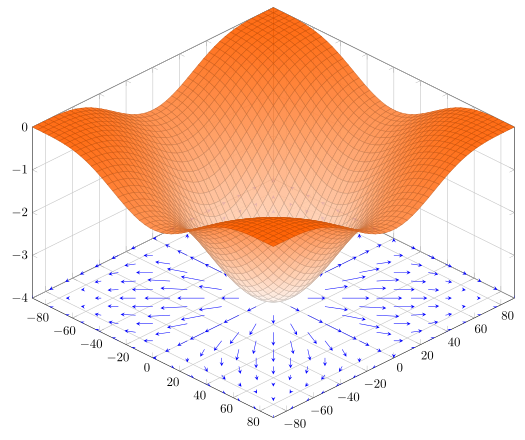
\includegraphics[width = 0.7 \linewidth]{1911.png}
    \caption{Độ dốc của hàm $f(x,y) = -(\cos^{2}{x}+\cos^{2}{y})^{2}$ được biểu diễn dưới dạng trường vector hình chiếu trên mặt phẳng đáy.}
    \label{fig1}
\end{figure}
\phantom{a}\\
Trong phạm vi bài này tôi chỉ giới thiệu đến đây, ta sẽ đi sâu hơn vào Gradient trong các bài học sau!
\subsection{Quy tắc dây xích - Chain Rule}
Ta đã biết trong thực tế, đôi khi các hàm số vị lồng vào nhau, khi đó ta gọi chúng là các hàm hợp, để đạo hàm được biến của hàm này qua hàm kia đôi khi là bất khả thi nếu theo lối mòn đã biết. Để phục vụ cho điêu đó, một quy tắc đã được ra đời để tối ưu hóa việc làm này, đó là quy tắc chuỗi/ quy tắc dây xích!
\begin{equation}
    \nabla_{\textbf{x}} g(f(\textbf{x}) = \nabla_{\textbf{x}}{f}^{T} \nabla_{f}{g}
\end{equation}
\subsection{Khai triển Taylor}
\label{n2}
\fbox{
\begin{minipage}{\linewidth}
    Cho $f$ là hàm số xác định trên miền mở $U$ với các đạo hàm riêng liên tục tới cấp m. Nếu \textbf{a} là điểm trong $U$ \textbf{h} là một vector trong $\mathbb{R}^{n}$ sao cho với với mọi $t \in [0,1]$ $\textbf{a} + t \textbf{h} \in U$, thì tồn tại số $\tau \in (0,1)$ thỏa mãn:
    \begin{equation}
        f(\textbf{a}+\textbf{h}) = f(\textbf{a})+\frac{F'(0)}{1!}+\frac{F''(0)}{2!}+\ldots+\frac{F^{(m-1)}(0)}{(m-1)!}+\frac{F^{m}(\tau)}{m!}
    \label{eq3}
    \end{equation}
    Trong đó $F(t) = f(\textbf{a}+t\textbf{h})$
\end{minipage}
}\\\\
Để tính được các đạo hàm trong công thức tên ta sẽ sử dụng quy tắc chuỗi. Trong trường hợp này, khá đơn giản ta có:
$$F'(t) = \nabla {f(\textbf{a}+t\textbf{h})^{T}.\textbf{h}}$$
Ví dụ, ta sẽ tính các lân cận của $f(x,y)$ thông qua khai triển Taylor.\\
$f(x+1,y+1) = f(x,y)+f'_{x}(x,y)+f'_{y}(x,y)$\\
$f(x-1,y-1) = f(x,y)-f'_{x}(x,y)-f'_{y}(x,y)$\\
$f(x+1,y-1) = f(x,y)+f'_{x}(x,y)-f'_{y}(x,y)$\\
$f(x-1,y+1) = f(x,y)-f'_{x}(x,y)+f'_{y}(x,y)$\\
$f(x,y+1) = f(x,y)+f'_{y}(x,y)$\\
$f(x,y-1) = f(x,y)-f'_{y}(x,y)$\\
$f(x+1,y) = f(x,y)+f'_{x}(x,y)$\\
$f(x-1,y) = f(x,y)-f'_{x}(x,y)$\\\\
Từ đây, tùy vào lượng lân cận mà ta cần, ta có thể tính các đạo hàm riêng của một hàm số tại một điểm bất kì!\\
ví dụ:
\begin{equation}
    \begin{aligned}
    8f'_{x}(x,y) &= f(x+1,y+1)-f(x-1,y-1)+f(x-1,y+1)-f(x+1,y-1)\\&\phantom{=}+2f(x,y+1)-2f(x,y-1)\\
    &=f\left(\begin{bmatrix}
        -1&0&1\\
        -2&0&2\\
        -1&0&1
    \end{bmatrix}\right)
    \end{aligned}
    \label{eq4}
\end{equation}
Đó chính là toán tử Sobel size 3x3 (\textit{Sobel Operator})! Ta sẽ sử dụng nhiều đến toán tử này cho các tác vụ đạo hàm riêng phần! Một cách tương tự, ta có toán tử Sobel size 3x3 cho theo phương y:
$$\begin{bmatrix}
    1&2&1\\
    0&0&0\\
    -1&-2&-1
\end{bmatrix}$$
\section{Theory of Edge Detection}
\subsection{Edge of Image}
Cạnh của ảnh là gì?\\
Như đã giới thiệu trong bài đầu tiên, ảnh số là tập hợp các pixels có giá trị: có thể là một vô hướng hoặc một vector. Ta có nhận xét rằng cạnh là những pixels mà lân cận của nó thay đổi đột ngột so với nó! (Hình \ref{fig2})\\\\
\begin{figure}[ht!]
    \centering
    \begin{subfigure}[b]{0.4\linewidth}
    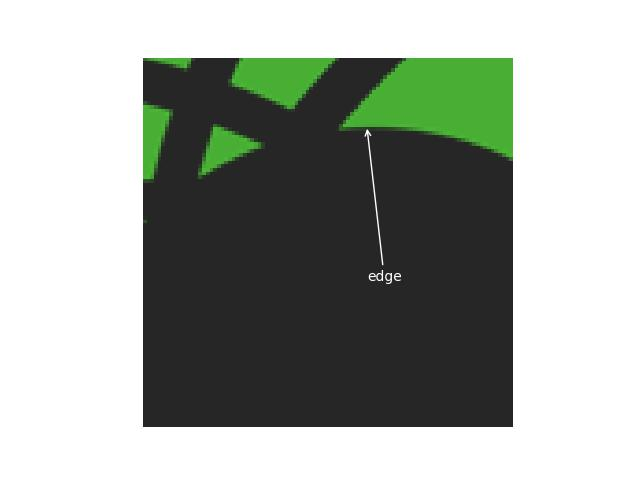
\includegraphics[width =\linewidth]{cut.jpg}
    \caption{Edge in Image Show}

    \end{subfigure}
    \begin{subfigure}[b]{0.5\linewidth}
    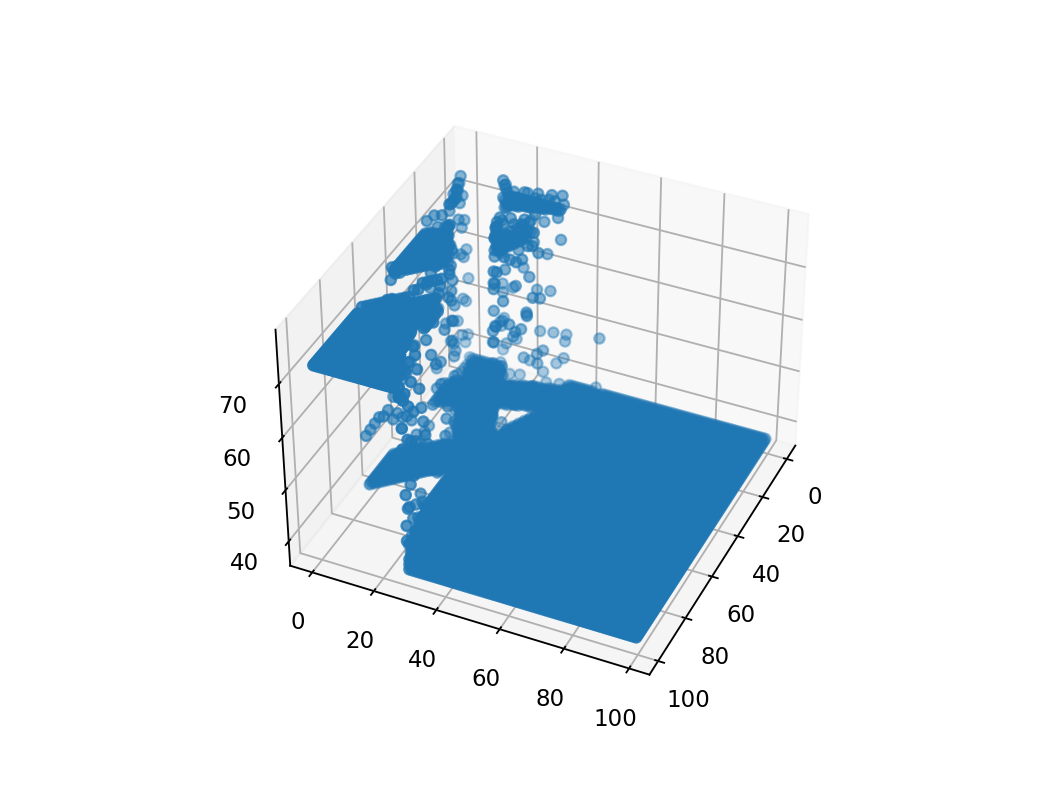
\includegraphics[width = \linewidth]{cut2.png}
    \caption{Edge in Plot show}
    \end{subfigure}
    \caption{Egde}
    \label{fig2}
\end{figure}Điều này vô hình lại trùng với khái niệm điểm uốn trong hàm số mà ta đã biết! Rõ ràng ta có cơ sở để xác định cạnh dựa trên những kiến thức về cực trị, điểm uôn, \ldots về mặt toán học!\\\\
Theo định nghĩa, điểm uốn là điểm mà đạo hàm bậc hai tại đó bằng 0. Tức là đạo hàm bậc nhất tại đó đạt cực trị. Đến đây ta hai hướng để xác định cạnh:
\begin{enumerate}
    \item Theo đạo hàm bậc nhất
    \item Theo đạo hàm bậc hai
\end{enumerate}
\section{Gradient of Image}
Như đã chúng ta đã biết, hình ảnh là tín hiệu rời rạc, hai chiều. Do đó so với các khái niệm đã thảo luận trong phần \ref{n1}. Ta có thể tóm gọn lại như sau:
\begin{enumerate}
    \item Gradient equation: $\nabla f= [\frac{\partial f}{\partial x}; \frac{\partial f}{\partial y}]$
    \item Gradient direction $\theta = \arctan{\left(\frac{\partial f}{\partial x}/ \frac{\partial f}{\partial y} \right)}$
    \item Gradient magnitude $||\nabla f|| = \sqrt{\left(\frac{\partial f}{\partial x}\right)^{2}+ \left(\frac{\partial f}{\partial y}\right)^{2}}$
\end{enumerate}
\section{Edge Detection}
    Như ta đã học ở \textit{Giải tích hàm nhiều biến}, để đi tìm cực trị của một hàm nhiều biến ta cần phải tìm các điểm dừng (giải hệ phương trình các đạo hàm riêng). Tương tự như vậy, ta sẽ tìm đạo hàm của ảnh theo phương x, và đạo hàm của ảnh theo phương y. Sẽ là tốt hơn nếu ta tổng hợp hai kết quả lại bằng \textit{Gradient magnitude}.\\ \\
 Từ đây ta có thể đưa ra các bước cơ bản để xác định được cạnh của một bức ảnh:\begin{enumerate}
     \item Tiền xử lí
     \item Tính Gradient của ảnh (Tính Đạo hàm của ảnh theo phương x và y)
     \item Tính Magnitude của Gradient
     \item Hậu xử lí
 \end{enumerate} 
 Hai bước đầu và cuối, là hai bước mở. Có thể có hoặc không, có thể ảnh hưởng hoặc ảnh hưởng rất nhiều đến thuật toán xác định cạnh!\\
 Ví dụ, đôi khi tín hiệu của ta là một tín hiệu nhiễu, ta vẫn xác định được cạnh một cách thủ công, nhưng không thể sử dụng các cách xấp xỉ đạo hàm! (Hình \ref{fig3})
 \begin{figure}[ht!]
     \centering
     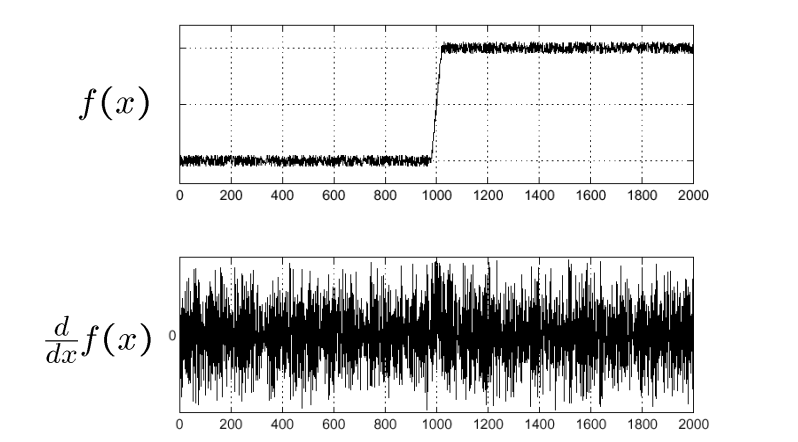
\includegraphics[width = 0.9\linewidth]{fig3.png}
     \caption{Noise Sensitive}
     \label{fig3}
 \end{figure}
 \phantom{a}\\
 Do đó giải pháp là các bước tiền xử lí thường là các bước làm mịn (\textit{Smooth}) (Hình \ref{fig4}). 
  \begin{figure}[ht!]
     \centering
     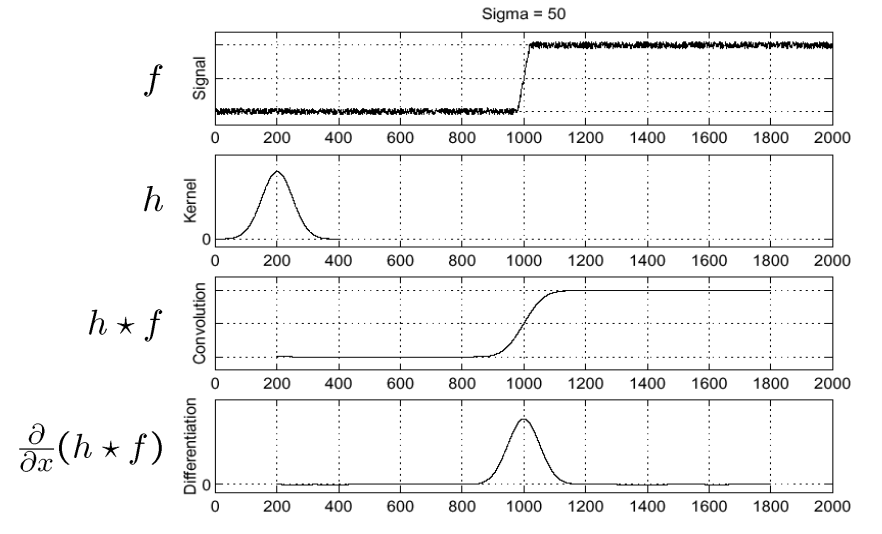
\includegraphics[width = 0.7\linewidth]{fig4.png}
     \caption{Smooth First}
     \label{fig4}
 \end{figure}
 \phantom{a}\\
 Còn các bước hậu xử lí, thường sẽ được chú trọng nhất. Bởi tất cả các bước trên là các bước cơ bản mà thuật toán xác định cạnh nào cũng cần. Nhưng bước hậu xử lí, gọi là hậu xử lí cũng không hoàn toàn đúng, đây là bước sẽ quyết định một thuật toán mới và sự thành công của thuật toán! Ví dụ thuật toán Canny, hay Hough Transform, \ldots (Ta sẽ thảo luận sau).\\\\
 Tạm gác lại hai bước trên, trước tiên ta cần thực hiện được hai bước cơ bản, thiết yếu ở giữa. Trước hết để tính được Gradient của ảnh, ta cần tính được các đạo hàm riêng phần của ảnh. Như đã giới thiệu ở trên (phần \ref{n2}). Đạo hàm của ảnh xuất phát từ ý tưởng sấp xỉ đạo hàm từ các lân cận của nó. Tùy vào các lân cận mà ta muốn sử dụng ta có các cách khác nhau để sấp xỉ đạo hàm, với toàn bộ bức ảnh toán tử đạo hàm có thể thay thế bằng phép tích chập giữa ảnh gốc và bộ lọc (xây dựng từ các lân cận). \\\\Ta có thể kể ra một số bộ lọc nổi tiếng như: Roberts (2x2), Sobel (5x5), Prewitt (3x3), \ldots Tuy nhiên phổ biến nhất vẫn là Sobel (3x3). Khi đó các đạo hàm riêng có thể được tính như sau:
        $$
   G_x = \begin{bmatrix}
        -1 & 0 & 1\\
        -2  & 0 & 2\\
        -1 & 0 & 1
    \end{bmatrix}*A
    \hspace{0.2\textwidth}
    G_y = \begin{bmatrix}
    1 & 2 & 1\\
    0 & 0 & 0 \\
    -1 & -2 & -1
    \end{bmatrix}*A
    $$
    Sở dĩ, toán tử Sobel được sử dụng phổ biến là vì bản thân nó ngoài xác định đạo hàm riêng của ảnh, nó còn kiêm làm mịn ảnh. Thực tế các công thức trên có thể được viết lại:
    $$G_x = \begin{bmatrix}
        1\\2\\1
    \end{bmatrix}*(\begin{bmatrix}
        1&0&-1
    \end{bmatrix}*A)\hspace{0.1\textwidth}     G_y = \begin{bmatrix}
        1\\0\\-1
    \end{bmatrix}*(\begin{bmatrix}
        1&2&1
    \end{bmatrix}*A)$$
    Sau đó sử dụng $$G = \sqrt{G_x^{2}+G_y^{2}}$$ ta hoàn thành bước 3. (Hình \ref{fig6})\\
    \begin{figure}[ht!]
        \centering
        \begin{subfigure}[b]{0.4\linewidth}
        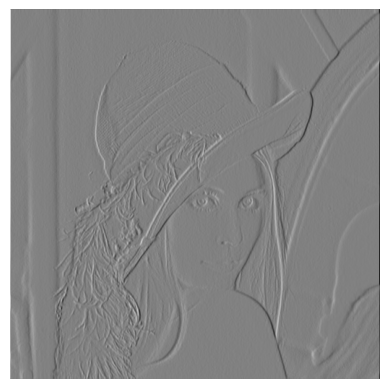
\includegraphics[width = \linewidth]{gx.png}
        \caption{$G_x$}
        
        \end{subfigure}
        \begin{subfigure}[b]{0.4\linewidth}
        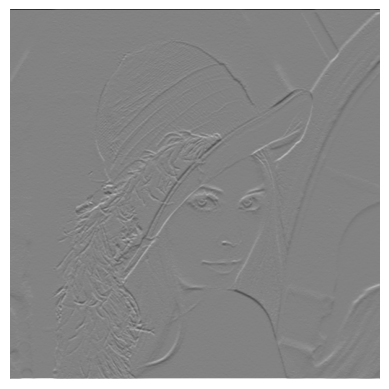
\includegraphics[width = \linewidth]{gy.png}
        \caption{$G_y$}
        
        \end{subfigure}
        
        \begin{subfigure}[b]{0.4\linewidth}
        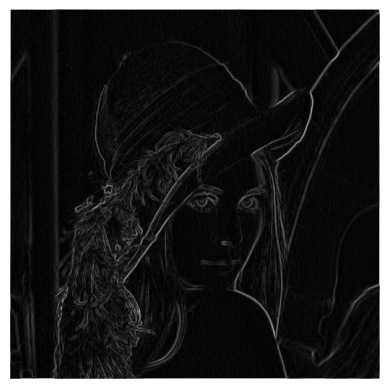
\includegraphics[width = \linewidth]{g.png}
        \caption{$G$}
        
        \end{subfigure}
        \caption{Gradient of Image}
        \label{fig6}
    \end{figure}\phantom{a}\\
    Bên cạnh cách xác định thông qua Gradient của ảnh, ta vẫn còn một cách khác như đã nói ở trên, đó là tính đạo hàm bậc hai của ảnh sau đó đi tìm các điểm làm đạo hàm bậc hai bằng không (\textit{zero-crossing}). Có thể kể đến các phương pháp như Laplacian, hay LoG,\ldots Nhưng không phổ biến bằng cách trên! (Các cách này thực hiện được chủ yếu nhờ tính đơn giản của bộ lọc và một kết luận sau đây!)
    \subsection*{Derivative Theorem of Convolution}
    Ta có kết quả sau đây:
    \begin{equation}
        \frac{\partial}{\partial x} (h*f) = \left(\frac{\partial}{\partial x} h\right)*f
    \end{equation}
    \underline{Chứng minh}:\\
    Dưới đây là chứng minh chỉ mang tính ý tưởng! Ta sử dụng Quy tắc Leibniz (\href{https://en.wikipedia.org/wiki/Leibniz_integral_rule#General_form:_Differentiation_under_the_integral_sign}{Leibniz's integral rule - Wiki})
    $$
    \begin{aligned}
\frac{\partial}{\partial x}(h*f)&= \frac{\partial}{\partial x} \int_{-\infty}^{\infty} f(t)h(x-t)dt\\
&=\int_{-\infty}^{\infty} \frac{\partial}{\partial x} \left( f(t)h(x-t) \right) dt\\
&=\int_{-\infty}^{\infty} f(t) \frac{\partial}{\partial x} h(x-t) dt\\
&=\left(\frac{\partial}{\partial x} h \right)*f \quad \square\phantom{a} Q.E.D
    \end{aligned}
    $$
Điều này có ý nghĩa gì?\\
Ý nghĩa lớn chứ!!! Nó sẽ giúp ta giảm được một bước tính tích chập! Vì ở bước tiền xử lí ta sẽ phải \textit{smooth} tín hiệu sử dụng tích chập, nhưng giờ ta có thể gộp việc \textit{smooth} với bước tính đạo hàm. Khi đấy số bước của ta chỉ còn là 3. (Hình \ref{fig5})
\begin{figure}[ht!]
    \centering
    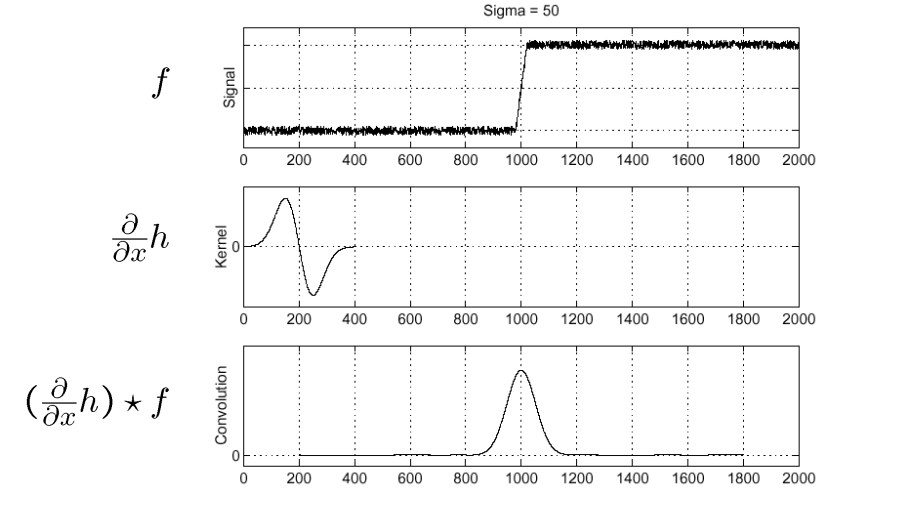
\includegraphics[width = 0.9\linewidth]{fig5.png}
    \caption{Reduce one step}
    \label{fig5}
\end{figure}
\phantom{a}\\
Hơn nữa việc lại là cực kì thuận lợi cho những thuật toán với ý tưởng phức tạp. Chẳng hạn như ý tưởng với zero-crossing. Bây giờ thay vì ta đạo hàm bậc hai cả ảnh ta chỉ cần đạo hàm bậc hai bộ lọc (việc này hoàn toàn làm thủ công được, rồi thay công thức cho máy tính). (Phần \ref{n3})
\\\\
Sau đây là một số thuật toán xác định cạnh cơ bản
\subsection{Laplacian of Gaussian - LoG}
\label{n3}
Thuật toán này còn được biết đến là Marr-Hildreth Detection.
Ý tưởng rất đơn giản: Đạo hàm bậc hai của hàm Gauss:
$$LoG = (2\pi \sigma^{2})\frac{(x^{2}+y^{2}-(2\sigma^{2})}{\sigma^{4}} \exp\{-(x^{2}+y^{2})/(2\sigma^{2})\}$$
Các bước có thể hình dung trong hình \ref{fig7}
\begin{figure}[ht!]
    \centering
    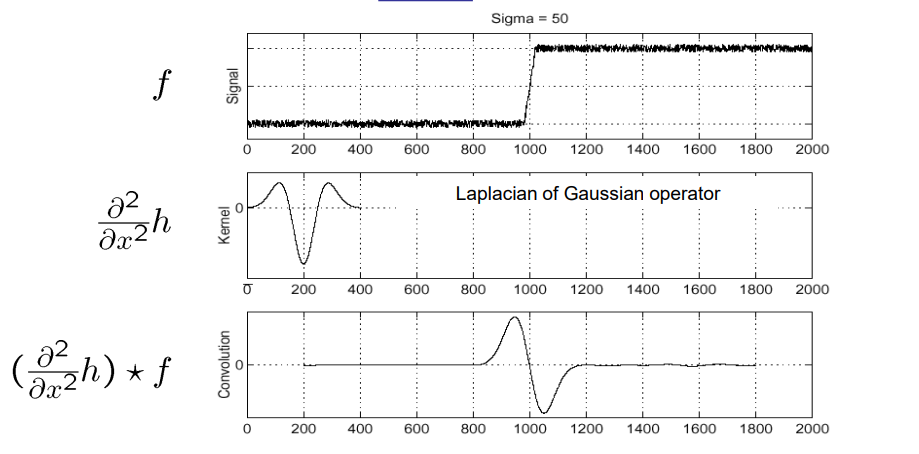
\includegraphics[width = 0.9\linewidth]{fig7.png}
    \caption{LoG Steps}
    \label{fig7}
\end{figure}
    \begin{figure}[ht!]
        \centering
        \begin{subfigure}[b]{0.4\linewidth}
        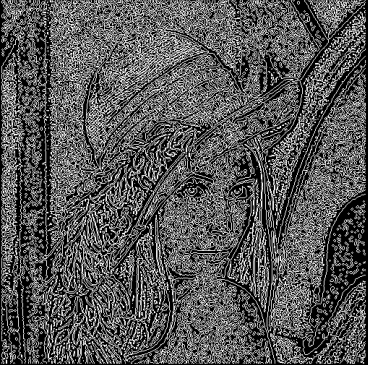
\includegraphics[width = \linewidth]{fig7a.png}
        \caption{Result}
        
        \end{subfigure}
        \begin{subfigure}[b]{0.4\linewidth}
        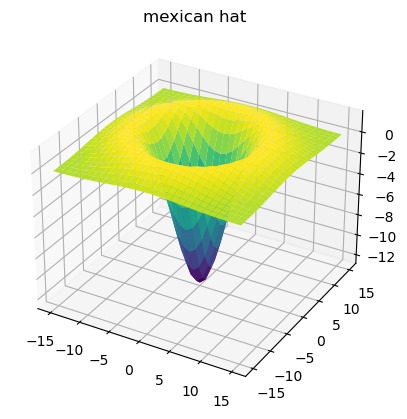
\includegraphics[width = \linewidth]{fig7b.png}
        \caption{LoG Filter - 
A Mexican hat}
        
        \end{subfigure}
        
        \caption{LoG Detection}
        \label{fig8}
    \end{figure}
    \phantom{a}\\\\
    Thuật toán này khá hiệu quả. Đây là thuật toán gọi là \textit{hot} vào thời điểm nó được đề xuất \ldots Cho đến khi một thuật toán khác hay hơn, hiệu quả hơn ra đời: \textit{Canny Detection}.
    \subsection{Canny Edge Detection}
    Đây là thuật toán hay, phổ biến và nhiều ứng dụng rộng rãi cho tận đến hiện tại. Với ý tưởng cơ bản là hậu sử lí Gradient của ảnh sao cho các cạnh `mảnh' nhất có thể! Hiển nhiên, điều này không hề dễ, ta có thể tóm gọn thuật toán Canny với các bước sau:
    \begin{enumerate}
        \item Noise reduction
        \item Gradient calculation
        \item Non-maximum Suppression
        \item Double Threshold
        \item Edge Tracking by Hysteresis
    \end{enumerate}
    Sau đây ta sẽ đi vào từng bước cụ thể!
    \subsubsection{Noise reduction}
    Bước này đơn giản là làm mịn. Như đã nói ở trên, đôi khi ở bước tính đạo hàm, chúng có thể bị nhạy cảm với nhiễu dẫn đến hoạt động không hiệu quả. Do đó, ta cần khử nhiễu trước khi tính Gradient của ảnh. \\\\
    Thường người ta sẽ sử dụng bộ lọc Gauss cho tác vụ này!\\\\
    Đôi khi bước này cũng có thể bỏ qua, nhưng phải đảm bảo ảnh/tín hiệu nhiễu ở mức độ chấp nhận được. Bởi đôi khi, làm mờ ảnh, cũng có thể dẫn đến mất đi nhiều chi tiết quan trọng.
    \subsubsection{Gradient calculation}
    Bước này là tính Gradient của ảnh như đã đề cập ở trên, thông qua $G_x$ và $G_y$ ta tính $G = \sqrt{G_x^2+G_y^2}$
    \begin{figure}[ht!]
        \centering
        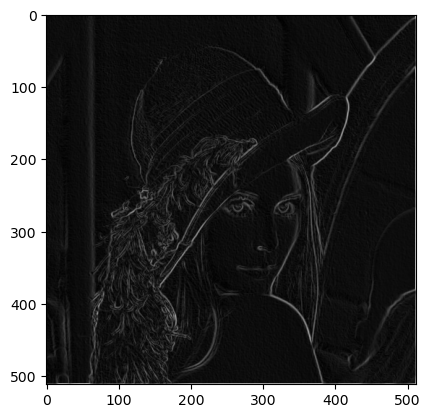
\includegraphics[width = 0.5\linewidth]{fig8.png}
        \caption{Gradient calculation step}
        \label{fig9}
    \end{figure}
    \subsubsection{Non-maximum Suppression}
    Như đã biết kết quả của Canny sẽ cho ra ảnh có cạnh mảnh. Do đó, ta sẽ cho
    thuật toán đi qua tất cả các pixel trên ảnh gradient và tìm các pixel có giá trị tối đa theo hướng cạnh.\\
    \begin{figure}[ht!]
        \centering
        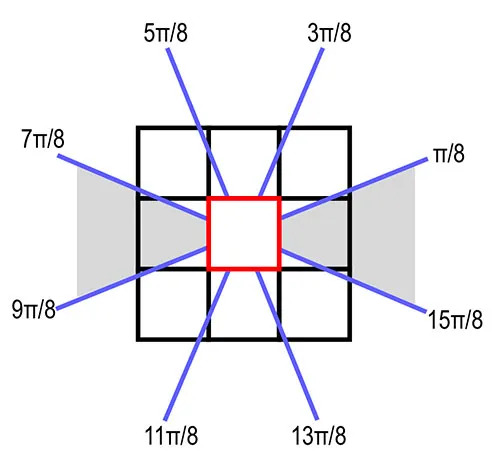
\includegraphics[width = 0.5\linewidth]{fig9.jpg}
        \caption{Gradient Directions}
        \label{fig10}
    \end{figure}\phantom{a}\\
    Ta đã có hướng Gradient $\theta = \arctan (G_x/G_y)$ như đã đề cập ở trên.  Dựa vào hướng đó ta sẽ xác định lân cận cho điểm mà ta đang duyệt, sau đó so sánh chúng. Nếu điểm ta đang xét, lớn hơn lân cận của chúng thì ta sẽ lưu lại vào ảnh mới, không thì ta sẽ bỏ qua.\\\\
    \underline{Lưu ý:} Về lí thuyết hướng Gradient có thể quay 360 độ, nhưng thực tế ta chỉ cần 180 độ, vì tính đối xừng của chúng và thực tế là ta cũng không làm việc với hướng mà hướng chỉ là cơ sở để ta xác định lân cận mà thôi. Nên thay vì 8 trường hợp như hình \ref{fig10} ta chỉ cần 4 trường hợp!\\\\
    \underline{Ví dụ}: Giả sử góc $\theta$ tại điểm $(h,v)$ của ta nằm trong $[0,22.5) \text{ or } [157.5, 180)$ tương đương hướng của Gradient là 0 độ hoặc 180 độ. Khi đó lân cận cần xét của $(h,v)$ là $(h,v+1)$ và $(h,v-1)$.
    \begin{figure}[ht!]
        \centering
        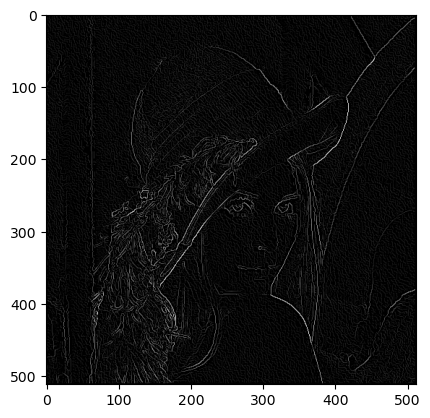
\includegraphics[width = 0.5\linewidth]{fig10.png}
        \caption{Non-maximum Supression step}
        \label{fig11}
    \end{figure}
    \subsubsection{Double Threshold}
    Phân ngưỡng kép! Ở bước này ta sẽ đưa ra hai ngưỡng \textit{MaxVal} và \textit{MinVal}. Khi đó xảy ra ba trường hợp cho một pixel:
    \begin{enumerate}
        \item Giá trị lớn hơn MaxVal: Chắc chắn là một cạnh. Set giá trị = 255
        \item Giá trị nằm trong khoảng MinVal và Maxval: Có thể là một cạnh (cạnh yếu). Set giá trị bằng một số nào đó (ví dụ = 50).
        \item Giá trị nhỏ hơn MinVal: Không phải cạnh. Set giá trị = 0.
    \end{enumerate}
    \begin{figure}[ht!]
        \centering
        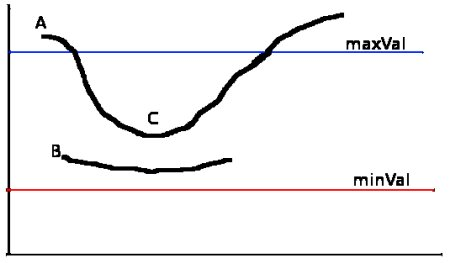
\includegraphics[width = 0.7\linewidth]{fig11.jpg}
        \caption{Double Threshold}
        \label{fig12}
    \end{figure}
    \begin{figure}[ht!]
        \centering
        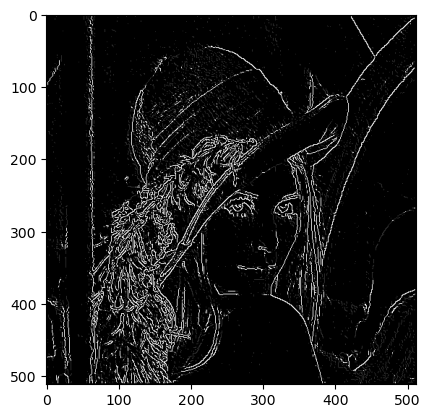
\includegraphics[width = 0.5\linewidth]{fig12.png}
        \caption{Double Threshold step}
        \label{fig13}
    \end{figure}
    \subsubsection{Hysteresis}
    Bước `trễ'. Như cái tên, ở bước này ta sẽ tiếp tục cho thuật toán chạy, ở đó ta sẽ xét những pixel mà ta đã cho rằng có thể là cạnh ở bước trên (cạnh yếu). Nếu lân cận của điểm đó, tồn tại một pixel chắc chắn là cạnh (cạnh mạnh) thì điểm đó sẽ được xét là cạnh (set giá trị = 255).
    \begin{figure}[ht!]
        \centering
        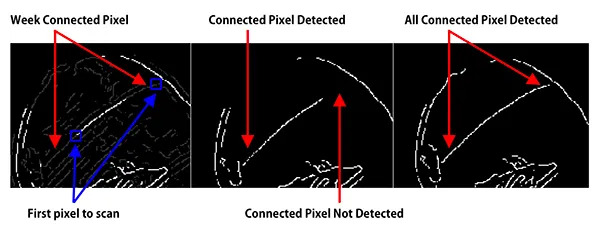
\includegraphics[width = 0.7\linewidth]{fig13.jpg}
        \caption{Notice}
        \label{fig14}
    \end{figure}
    \phantom{a}\\
    Nhìn vào hình \ref{fig14}. Ta cần lưu ý: Ở bước này, để đạt được hiệu quả tốt nhất ta cần duyệt ảnh theo 4 phương chứ không phải là một phương như bình thường ta hay làm (\textit{tức là duyệt từ trái sang phải, từ trên xuống dưới}). Vì sẽ xảy ra trường hợp các cạnh yếu được xếp gần nhau nhưng chỉ có một phía cạnh yếu được xếp cần cạnh mạnh, nếu phía đấy không phải phía được duyệt qua trước thì đen. Khi đó phần lớn các cạnh yếu sẽ bị bỏ qua. Tuy nhiên, việc làm này khá mất thời gian, tôi cũng chỉ làm một hướng mà thôi :)). Để tìm hiểu kĩ hơn bạn có thể tham khảo ở đây:
    \href{https://www.adeveloperdiary.com/data-science/computer-vision/implement-canny-edge-detector-using-python-from-scratch/}{Implement Canny edge detector using Python from scratch - adeveloperdiary.com}
    \begin{figure}[ht!]
        \centering
        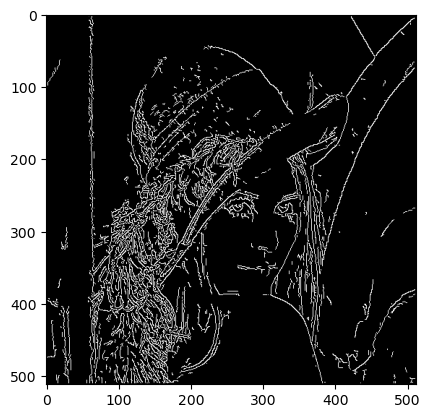
\includegraphics[width = 0.5\linewidth]{fig14.png}
        \caption{Hysteresis step}
        \label{fig15}
    \end{figure}
    \subsection{Hough Transform Detection}
    Đây là thuật toán khá thú vị, ra đời để giải bài toán: Xác định các dạng hình học cơ bản trên một bức ảnh: Đường thẳng, đường tròn, elipse, \ldots Trong nghiên cứu về xe tự hành, đây hẳn là thuật toán không thể thiếu, bởi tính đơn giản, hiệu quả của nó! Trong phạm vi bài này, tôi sẽ chỉ giới thiệu về thuật toán xác định đường thẳng, các thuật toán còn lại có thể làm tương tự!
    \subsubsection{Đường thẳng}
    Như đã biết một đường thẳng trong hệ tọa độ \textit{Descartes} đươc cho bởi phương trình tổng quát sau: $y = ax+b$. Rõ ràng với bộ số $(a,b)$ ta đã có một đường thẳng! Thật vậy ta gọi một không gian mới \textit{Hough Coordinate}, ta thiết lập được một song ánh giữa hệ tọa độ \textit{Hough} và hệ tọa độ \textit{Descartes}, ở đó một điểm tương đương với một đường thẳng, tương tự một đường thẳng tương đương một điểm trong hệ tọa độ \textit{Descartes}. (Hình \ref{fig16})
    \begin{figure}[ht!]
        \centering
        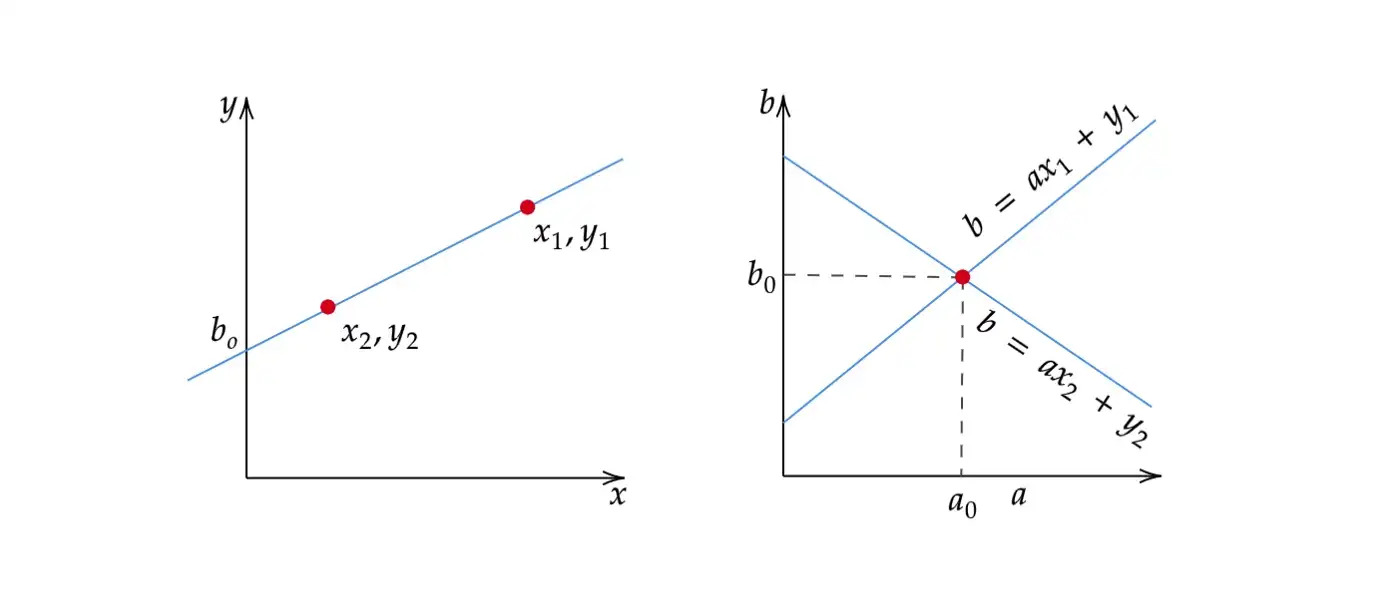
\includegraphics[width = 0.7\linewidth]{fig15.jpg}
        \caption{Mapping from edge points to the Hough Space.}
        \label{fig16}
    \end{figure}
    \phantom{a}\\
    Tuy nhiên với song ánh trên thì $a, b$ của ta vô hạn, việc này là khó khăn trong việc kiểm soát về mặt giới hạn! Nên ta sẽ thiết lập một ánh xạ khác! 
    \begin{figure}[ht!]
        \centering
        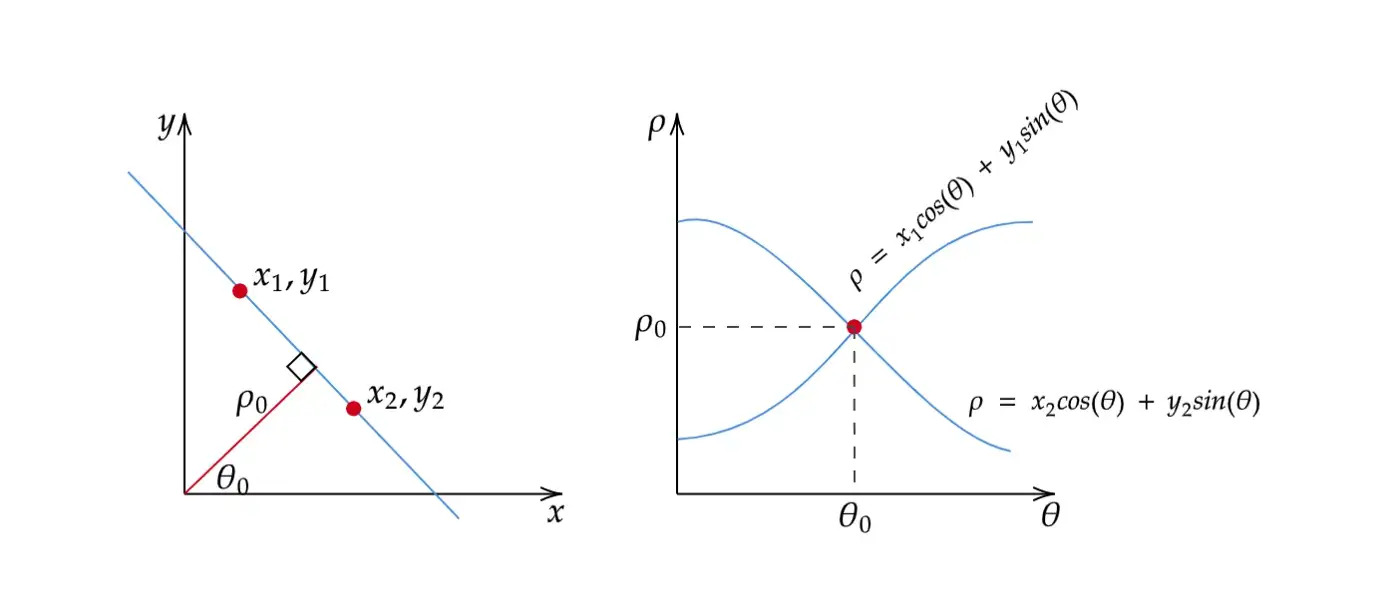
\includegraphics[width = 0.7\linewidth]{fig16.jpg}
        \caption{An alternative representation of a straight line and its corresponding Hough Space.}
        \label{fig17}
    \end{figure}
    \phantom{a}\\
    Nếu ta gọi $\rho$ là khoảng cách từ gốc O đến đường thẳng. $\theta$ là góc tạo bởi đường thẳng đi qua O vuông góc với đường thẳng và trục Ox. Khi đó theo phương trình đoạn chắn ta có:
    $$\frac{x}{\frac{\rho}{\cos \theta}}+\frac{y}{\frac{\rho}{\sin \theta }} = 1$$
    Tương đương:
    \begin{equation}
         x \cos \theta + y \sin \theta = \rho
         \label{eq6}
    \end{equation}
    Khi đó ta có một song ánh mới giữa đường thẳng trong hệ tọa độ \textit{Descartes} đến một điểm $(\theta,\rho)$ trong hệ tọa độ \textit{Hough}. Song ánh này là dễ kiểm soát hơn nhiều, bởi $\rho$ luôn nhỏ hơn bằng đường chéo của bức ảnh, đồng thời $\theta$ luôn trong khoảng $[0, 360)$ độ.\\\\
    \underline{Lưu ý:} Hệ tọa độ với hai biến $(\rho,\theta)$ còn gọi là hệ tạo độ cực (\textit{polar coordinate system}). Và trong hệ tọa độ cực có một số lưu ý sau:
    \begin{enumerate}
        \item $\rho \geq 0, \forall \theta$
        \item $\theta \in [0, 2\pi)$ 
        \item Hệ tọa độ cực suy rộng: Nếu $\rho_1 <0$ ta định nghĩa $(\rho_1, \theta) = (-\rho_1,\theta + \pi)$
    \end{enumerate}
    \underline{Nhận xét:} Ta có nhận xét: Qua phép biến đổi \textit{Hough}, một đường thẳng bị biến thành một điểm, một điểm bị biến thẳng một đường. Do đó một đường thẳng trong hệ tọa độ \textit{Descartes} sẽ ứng với một điểm bị vô hạn đường thẳng cắt qua trong hệ tọa độ \textit{Hough}.\\\\
    Đến đây tôi tin bạn đọc cũng đoán được sương sương về ý tưởng của thuật toán này! Thuật toán này không khó, sau đây tôi sẽ tóm tắt lại các bước chính của thuật toán.
    \subsubsection{The Algorithm}
    Thuật toán xác định đường thẳng \textit{Hough} có thể chia làm các bước sau:
    \begin{enumerate}
        \item Xác định cạnh bức ảnh bằng thuật toán \textit{Canny}
        \item Xác định kích thước cho mảng tích lũy (\textit{accumulator}) (mảng dùng để xác định các đường thẳng, tức các giao điểm trong hệ tọa độ \textit{Hough}). Kích thước ở đây tức là độ dài, ngắn của các mảng sấp xỉ cho giá trị có thể có của $\rho, \theta$
        \item Tạo mảng tích lũy `không' (tất cả phần tử bằng 0) với các kích thước đã xác định ở trên
        \item Duyệt qua những \textit{pixel} là cạnh, tại đó ta duyệt tiếp $\theta$, tính $\rho$ theo công thức (\ref{eq6}). Xác định vị trí của cặp $(\theta,\rho)$ trong mảng tích lũy và tăng giá trị lên một mức (tùy chọn giá trị tăng)
        \item Cuối cùng là phân ngưỡng (\textit{Threshold}). Phân ngưỡng trên mảng tích lũy xem điểm nào có giá trị tích lũy lớn hơn ngưỡng thì lưu lại. Sau khi phân ngưỡng, với các giá trị cặp giá trị $(\theta, \rho)$ hoàn toàn có thể suy ngược lại được phương trình tổng quát của đường thẳng cần xác định!
    \end{enumerate}
    Thuật toán khá rõ ràng và dễ hiểu. \\\\
    \underline{Lưu ý:} Như đã nói ở trên $\theta$ của ta nằm trong $[0^o,360^o)$. Tuy nhiên thực tế ta chỉ cần $3/4$ góc phần tư, hoàn toàn có thể bỏ qua góc phần tư thứ ba tức là khoảng $[180^o,270^o)$ (Xin nhường bạn đọc kiểm chứng và chứng minh).
    \begin{figure}
        \centering
        \begin{subfigure}[b]{0.7\linewidth}
            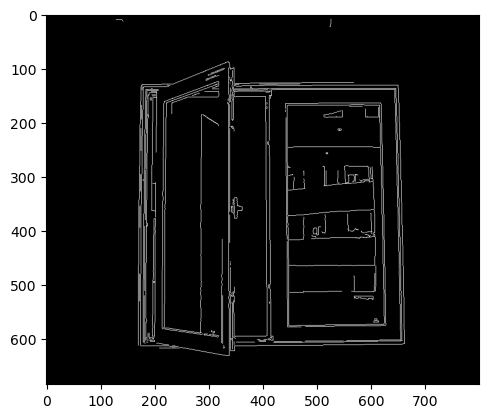
\includegraphics[width = \linewidth]{fig18a.png}
            \caption{Canny Step}
        \end{subfigure}

        \begin{subfigure}[b]{0.7\linewidth}
            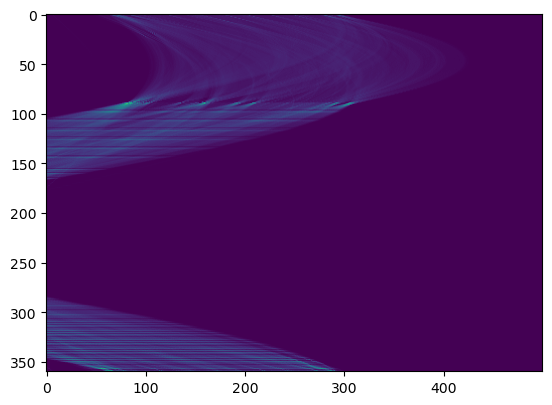
\includegraphics[width = \linewidth]{fig18b.png}
            \caption{Accumulator}
        \end{subfigure}

        \begin{subfigure}[b]{0.7\linewidth}
            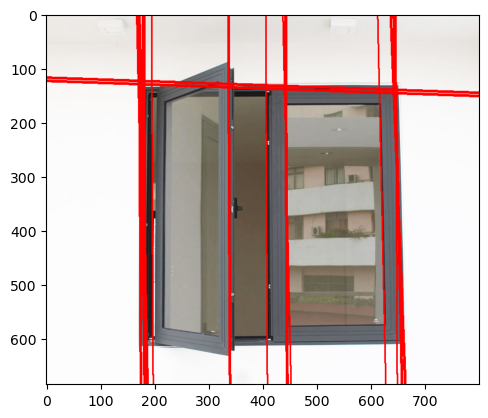
\includegraphics[width = \linewidth]{fig18c.png}
            \caption{result}
        \end{subfigure}
        
        \caption{Hough Line Transform Detection}
        \label{fig18}
    \end{figure}
    \subsubsection{Bàn luận}
    Với ý tưởng tương tự ta có thể làm cho các loại hình học cơ bản khác, miễn là có phương trình tổng quát và kiểm soát được các giới hạn độ lớn của chúng.\\\\
    Ví dụ: Đường tròn có phương trình tổng quát: $(x-a)^2+(y-b)^2 = r^2$. Có ngay điểm tương ứng trong không gian ba chiều \textit{Hough} $(a,b,r)$. Lần này chẳng cần phải chuyển sang tọa độ cực đâu, do $a,b$ bị giới hạn bởi chiều dài, chiểu rộng, thậm chí $r$ cũng bị giới hạn bởi chiều rộng.\\\\
    Hoàn toàn tương tự về mặt thuật toán!\\\\
    \underline{Song:} Hạn chế chính là độ phức tạp thuật toán, do phải duyệt nhiều biến, nên kích thước ảnh càng lớn, phương trình hình học càng phức tạp, rồi kích thước mảng tích lũy lớn nữa thì thuật toán là không hiệu quả. Tôi đã không thành công trong ngay trường hợp đường tròn (chạy thử trên cpu)!
    \subsubsection*{Đề xuất:} Hiện tại tôi cũng chỉ dám đưa ra đề xuất, cũng tạm thời chưa có thời gian để thực hiện. Hi vọng, thời gian tới, học nhiều cái mới, tiếp thu được nhiều kiến mới, kết hợp với những đề xuất này tôi sẽ có kết quả tốt hơn!
    \begin{enumerate}
        \item Tiếp tục sử dụng tọa độ cực. Do kích thước $\theta$ là hơp lí và khá cố định, không phụ thuộc vào ảnh đầu vào
        \item Chọn kích thước mảng tích lũy hợp lí. Thực tế cho tôi thấy rằng kích thước mảng tích lũy bé vẫn cho kết quả khá hợp lí. Hình \ref{fig18} là một kết quả, tôi có để thông số, bạn đọc có thể tự so sánh
        \item Duyệt có lựa chọn (kiểu \textit{adaptive filter}), thẳng nào kích thước ít hơn thì duyệt trước
        \item :)) Cái này đặt trước cho tương lai vậy
    \end{enumerate}
    \underline{Lưu ý:} Chú ý khi duyệt, cần sử dụng thành thạo các thao tác như: \textit{where, zip, enumerate, \ldots}
    \subsubsection{Xác định đường thẳng}
    Ở đây có một thuật toán khá hay, tuy nhiên cũng chưa được tối ưu. Là một thuật toán mẫu trong Lab tôi, bạn đọc có thể tìm thấy ở các code Tuto. Hoặc tìm được ở link sau: \href{https://minhng.info/tutorials/phat-hien-doan-thang-hough-transform.html}{Phán hiện đoạn thẳng Hough Transform - minhng.info}.\\\\
    \subsubsection*{Ý tưởng:} Sau khi đã xác định được các đường thẳng. Ta duyệt theo từng đường thẳng, sau đó duyệt qua tất cả các cạnh, lưu các cạnh thuộc đường thẳng lại. Sắp xếp và sau đó thực hiện duyệt theo lân cận. Tức ta sẽ lưu lại một điểm gọi là điểm hiện tại rồi duyệt list các cạnh, xem điểm đó có phải điểm đầu hay điểm cuối của đoạn thẳng không. Nếu không thì ta chuyển cạnh hiện tại thành cạnh đang duyệt, và xét tiếp. Sau cùng thì ý tưởng cũng là đi tìm hai đầu mút và lưu lại.\\\\
    Kết quả khá tốt, song vẫn chưa hiệu quả như tác giả mong muốn. Muốn tìm hiểu kĩ hơn, xin đọc ở link đã gắn ngay bên trên.
    \subsubsection*{Đề xuất:} %Ý tưởng này tôi cũng chợt nghĩ ra thôi, đơn giản, duyệt nhanh, song chưa hiệu quả bằng. Đó là ta sử dụng một kết quả đơn giản: Một đầu mút chỉ có lân cận một phía!
    \section{Mã nguồn}
    Mã nguồn cho bài này có thể tìm thấy ở đây: \href{https://github.com/thuantn210823/Computer-Vision-IPSAL-LAB-/tree/main/week%207-8}{week 7-8}

    \newpage
\section{Tài liệu tham khảo}
    \begin{thebibliography}{9}
        \bibitem{slide}
        Truong. PV, Thao. TT \emph{Tutorial 2
        Image gradient \& Edge Detection}, Đại học Bách Khoa Hà Nội.
        \bibitem{slide}
        Thao. NX \emph{Bài 6: Các lược đồ khảo sát hàm số - Bài giảng Giải tích I cho hệ KSTN}, Đại học Bách Khoa Hà Nội.
        \bibitem{book}
        Tri. ND, Dinh. TV, Quynh. NH \emph{Toán học cao cấp tập hai: Phép giải tích một biến số}, Nhà xuất bản Giáo Dục.
        \bibitem{book}
        Luc. DT, Dien. PH, Phuong. TD \emph{Giải tích các hàm nhiều biến: Những nguyên lí cơ bản và tính toán thực hành}, Nhà xuất bản Đại học Quốc gia Hà Nội.
    \bibitem{website}
    \href{https://towardsdatascience.com/lines-detection-with-hough-transform-84020b3b1549}{Lines Detection with Hough Transform - towardsdatascience.com}.
    \bibitem{website}
    \href{https://docs.opencv.org/4.x/d4/d70/tutorial_hough_circle.html}{Hough Cirle Tutorial - docs.opencv.org}
    \bibitem{website}
    \href{https://www.adeveloperdiary.com/data-science/computer-vision/implement-canny-edge-detector-using-python-from-scratch/}{Implement Canny Edge Detector using Python from scratch - adeveloperdiary.com}.
    \bibitem{website}
    \href{https://docs.opencv.org/4.x/da/d22/tutorial_py_canny.html}{Canny tutorial - docs.opencv.org}.
    \bibitem{website}
    \href{https://towardsdatascience.com/canny-edge-detection-step-by-step-in-python-computer-vision-b49c3a2d8123}{Canny Edge Detection Step by Step in Python Computer Vision - owardsdatascience.com}
    \bibitem{website}
    \url{https://github.com/adl1995/edge-detectors/blob/master/marr-hildreth-edge.py}
    \bibitem{website}
    \href{https://en.wikipedia.org/wiki/Gradient}{Gradient - Wikipedia}
    \end{thebibliography}


\end{document}


